\documentclass{beamer}

%%% -------------- CREATE HANDOUTS -----------------------------------
%\documentclass[12pt, handout]{beamer}
%\usepackage{pgfpages}
%\pgfpagesuselayout{4 on 1}[letterpaper, landscape, border shrink=5mm]
%%% ------------------------------------------------------------------


\mode<presentation>
  \usepackage{ru}
  %\usetheme{Warsaw}
  %\usecolortheme{seahorse}
  %\usefonttheme{default}
  \setbeamertemplate{caption}[numbered]
  %\setbeamertemplate{navigation symbols}{}
  \setbeamertemplate{bibliography item}[text]
\newcommand*\oldmacro{}%
	\let\oldmacro\insertshorttitle%
%\renewcommand*\insertshorttitle{%
%   \oldmacro\hfill%
%   \insertframenumber\,/\,\inserttotalframenumber}
\setbeamertemplate{section page}{
    \begin{centering}
    \vspace{1cm}
    \begin{beamercolorbox}[rounded=true,shadow=false,sep=4pt,center]{part title}
    \usebeamerfont{section title}\LARGE{\insertsection}\par
    \end{beamercolorbox}
    \end{centering}}
\usepackage{ragged2e}
\usepackage[english]{babel}
\usepackage[utf8]{inputenc}
\usepackage{appendixnumberbeamer}
\usepackage{natbib}
\usepackage{textpos}
\usepackage{lipsum}
\usepackage{tikz}
\usepackage[percent]{overpic}
\usepackage{textcomp}
\usepackage{booktabs}
\usepackage{mathabx}
\usepackage{pifont}
\usepackage{bbding}
\usepackage{fontenc}
%\let\Sun\undefined   %to undefine something
%\usepackage{marvosym}
%\usepackage{scalerel}

\setbeamerfont{caption}{size=\tiny}

%\setbeameroption{show notes}
%\setbeamertemplate{note page}[plain]
\newcommand{\tss}{\textsuperscript}
\newcommand{\tsbs}{\textsubscript}
%Change Bullets in latex list
\setbeamertemplate{itemize item}{\scriptsize\raise1.25pt\hbox{\donotcoloroutermaths\ding{118}}}
\setbeamertemplate{itemize subitem}{\scriptsize\raise1.25pt\hbox{\ding{226}}}
\setbeamertemplate{itemize subsubitem}{\tiny\raise1.25pt\hbox{\ding{169}}}
\setbeamertemplate{enumerate item}{\insertenumlabel.}


%%To select specific font
%{\fontsize{2.5}{4}\selectfont tobesize}

%\setbeamertemplate{background}{\tikz[overlay, remember picture]\node[xshift=-2.3cm, yshift=1.50cm, opacity=0.4]at (current page.south east){
\includegraphics[width=4cm]{images}};}

\title[Decontamination Factors for Nuclear Forensics]{Characterizaiton of Pu Separation by PUREX}
\author{Paul Mendoza}
\date{September 28, 2016}

\begin{document}
\begin{frame}
	%% background
  \tikz[overlay, remember picture]\node[xshift=-3.5cm, yshift=3cm, opacity=0.1]at (current page.south east){
\includegraphics[width=8cm]{tamu_system_proposed_seal_042915}};
	%% Left-hand logo
  \begin{tikzpicture}[remember picture, overlay]
  \node [xshift = 3 cm, yshift=1.2cm] at (current page.south west){
\includegraphics[width=5cm]{tees_logo_primary_maroon}};
  \end{tikzpicture}
    %% Right-hand logo
  \begin{tikzpicture}[remember picture, overlay]
  \node [xshift = -3cm, yshift=1.2cm] at (current page.south east){
\includegraphics[width=5cm]{TEES_NSSPI_logo_HMaroon}};
  \end{tikzpicture}
  %% Upper logo right
    \begin{tikzpicture}[remember picture,overlay]
    \node[anchor=north east,yshift=2pt] at (current page.north east) {
\includegraphics[height=0.8cm]{cyclologo}};
    \end{tikzpicture}
    \begin{tikzpicture}[remember picture,overlay]
    \node[anchor=north west,yshift=2pt] at (current page.north west) {
\includegraphics[height=0.8cm]{NUENlogo}};
    \end{tikzpicture}
  
  \titlepage
\end{frame}

%Add Biola Seal
\setbeamertemplate{background}{\tikz[overlay, remember picture]\node[xshift=-2.5cm, yshift=2.5cm, opacity=0.05]at (current page.south east){
\includegraphics[width=6cm]{imageedit_2_7317234434}};}

%Add NSSPI to upper right
\addtobeamertemplate{frametitle}{}{%
  \begin{tikzpicture}[remember picture,overlay]
    \node[anchor=north east,yshift=2pt] at (current page.north east) {
\includegraphics[height=0.8cm]{TEES_NSSPI_Acronym_logo_WHT}};
    \end{tikzpicture}}



\begin{frame}{Outline}
\tableofcontents
\end{frame}

\section{Motivation}
\begin{frame}{Big Picture}
\begin{itemize}
\item{Pu isotopes produced in irradiated fuel can vary depending on}
  \begin{itemize}
  \item{Burnup (irradiation history)}
  \item{Reactor neutron spectrum (core design)}
  \end{itemize}
\item{Weapons-grade Pu can be extracted from reactor discharged fuel
  with a burnup of about 1 (GWD/tU)}
\item{Two examples of non-safeguarded reactors which can intentionally
  discharge low burned fuel for extracting weapon-grade Pu are:}
  \begin{itemize}
  \item{Indian Prototype Fast Breeder Reactor (PFBR-500MWe)}
    \note[item]{Madras Atomic Power Station Kalpakkam, India}
    \note[item]{Expected criticality in Jan 2017}
    \note[item]{Cost from 450 million euros to 750 euros}
    \note[item]{Sodium-cooled reactor design - U238 for breeding}
    \note[item]{100 GWd/t for core, 40 year life, 1750 tonnes of sodium
      about 75\% of olympic sized swimming pool.}
    \note[item]{liquid sodium has a density a little less than water}
    \note[item]{MOX fuel (UO2 and PuO2) fuel}
    \note[item]{Fuel discharged at 100GWd/t, but I just mentioned
      that we are worried about 1GWd/t, mistake?}
  \item{Indian Pressureized Heavy Water Reactor (PHWR-CANDU type 220 MWe)}
  \end{itemize}
\item{In accord with the Indo-US 123 agreement, these reactors were not
      required to be kept under IAEA safeguards}
\end{itemize}
\end{frame}

\begin{frame}{Smaller Picture}
  \begin{columns}
    \begin{column}{0.5\textwidth}
      \vspace{-3mm}
      \begin{itemize}
      \item{Attribution for unpurified Pu has been previously studied
        \tss{\cite{chirayath2015trace,scott2005nuclear,glaser2009isotopic}}}
      \item{Intercepted Pu would likely have been processed via PUREX}
      \item{Due to a lack of literature on decontamination factors and
        distribution coefficients for useful forensic elements (Cs, Sb,
        Eu, Rb, Sr, Nd, Pm, and Sm) this research was pursued.} 
      \end{itemize}
    \end{column}
    \begin{column}{0.5\textwidth}
      \begin{figure}[H]
        \vspace*{-0.3cm}
        \begin{center}
	   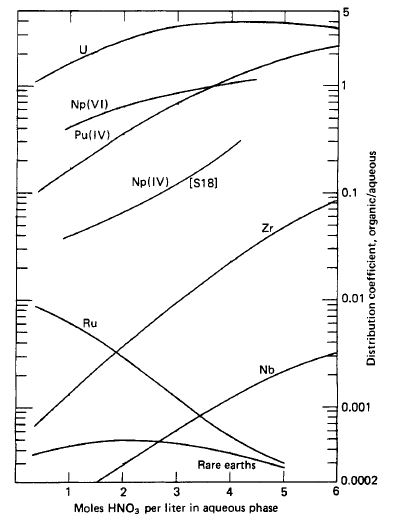
\includegraphics[scale = 0.4]{Stoller}
           \caption{\tiny{Effect of nitric acid concentration on
               distribution coefficients \tss{\cite{stoller1961reactor}}}}
	\end{center}
      \end{figure}
    \end{column}
  \end{columns}  
\end{frame}


\section{Background}
\begin{frame}
\sectionpage
\end{frame}

\subsection{The PUREX Process}
\begin{frame}{What is PUREX - A type of laundry detergent?}
  \vspace{0.5cm}
  \begin{itemize}
  \item Plutonium Uranium Redox EXtraction 
    \begin{itemize}
    \item Liquid-liquid solvent extraction
    \item Many stages:
      \begin{enumerate}
      \item{Preparation for Dissolution}
      \item{Dissolution}
      \item{Preparation of Dissolved Feed}
      \item{Primary Decontamination - Extraction to
        organic\textsuperscript{\tiny{\AsteriskThin}}}
      \item{Scrubbing}
      \item{Plutonium Partition - Back-Extraction to
        aqueous\textsuperscript{\tiny{\AsteriskThin}}}
      \item{Plutonium Purification}
      \end{enumerate}
    \end{itemize}
  \end{itemize}
  \vspace{1.5cm}
  \textsuperscript{\tiny{\AsteriskThin\hspace{1mm}- Discussing Next}}
\end{frame}


\begin{frame}{Extraction}
  \begin{figure}[H]
    \vspace*{0.1cm}
    \begin{center}
      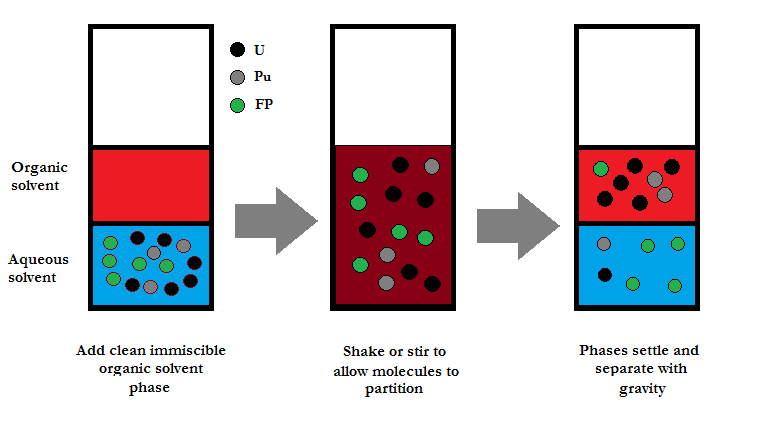
\includegraphics[scale = 0.5]{Extraction}
      \vspace{-0.7cm}
      \caption{\tiny{Extraction graphic}}
    \end{center}
  \end{figure}
\end{frame}

\begin{frame}{Back-Extraction}
  \begin{figure}[H]
    \vspace*{0.1cm}
    \begin{center}
      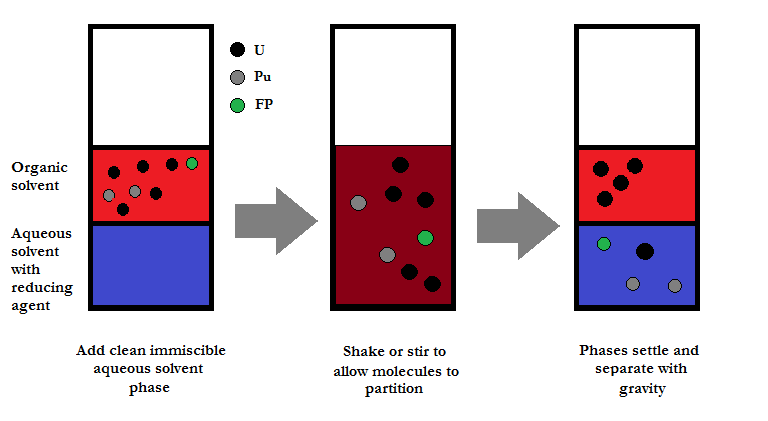
\includegraphics[scale = 0.5]{Back_Extraction}
      \vspace{-0.7cm}
      \caption{\tiny{Back-extraction graphic}}
    \end{center}
  \end{figure}
\end{frame}


\begin{frame}{Extraction and Back-extraction}
  \begin{columns}
    \begin{column}{0.5\textwidth}
      \vspace{-3mm}
      \begin{itemize}
      \item{Extraction}
        \\
        \scalebox{0.5}{$UO_2^{2+}(aq)+2NO^{-}_{3}(aq)+2TBP(o)
          \leftrightarrow UO_2(NO_3)_2\cdot2TBP(o)$\tss{\cite{benedict1982nuclear}}}
        \scalebox{0.5}{$Pu^{4+}(aq)+4NO^{-}_3(aq)+2TBP(o)
          \leftrightarrow Pu(NO_3)_4\cdot 2TBP(o)$}\\
        {\fontsize{2.5}{4}\selectfont Most of the fission products are
          left in the aqueous solution
        at valence III and V states\tss{\cite{kok2009nuclear}}}
      \item{Back-extraction}
        \begin{itemize}
          \scalebox{0.5}{$Pu(NO_3)_4(TBP)_{2_o}+Fe^{2+}_{aq}
            \leftrightarrow Pu^{3+}_{aq}+4NO^{-}_{3_{aq}}+2TBP_o$
            \tss{\cite{konings2006chemistry}}}
          \note[item]{The fission products that contribute mostly
            to the radioactive contamination of product in PUREX
            are zirconium, niobium, and ruthenium - with multiple
            oxidation states.}
        \end{itemize}
      \end{itemize}
    \end{column}
    \begin{column}{0.5\textwidth}
      \begin{figure}[H]
        \vspace*{-1cm}
        \begin{center}
	   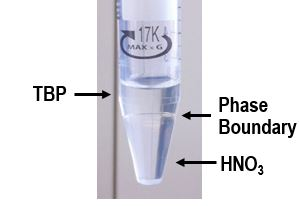
\includegraphics[scale = 0.75]{TBP2}
           \caption{\tiny{TBP and HNO$_3$}}
	\end{center}
      \end{figure}
    \end{column}
  \end{columns}  
\end{frame}

\subsection{Distribution Coefficients}
\begin{frame}{Distribution Coefficients - The Missing link}
  \begin{itemize}
  \item{Distribution Coefficient (DC): The ratio between the organic
  and aqueous phases}
    \begin{equation*}
      DR=\frac{c_{o}}{c_{aq}}
    \end{equation*}
    \note[item]{Distribution coefficients can be reported
      in terms of volume basis (weight per unit volume), or a
      mass basis (mass of solute per unit mass of solute free
      solvent)- usually reported on volume basis}
  \item{Specific element to element}
  \item{Vary widely with:\tss{\cite{stoller1961reactor}}}
    \begin{itemize}
    \item{Concentrations of solutions}
    \item{Saturation of U and Pu in the system}
    \item{Temperature of the solvents}
    \end{itemize}
  \item{The fraction of mass, $f_o$ deposited in the organic
    phase, assuming a volume ratio between
    the aqueous and organic phases, $V_R$, is:}
    \begin{equation*}
      f_o=(1+DC^{-1}V^{-1}_R)^{-1}
    \end{equation*}
    \note[item]{Note not a function of density, even though
      the two solutions have different densities, when solving for
      this value it cancels out}
    \note[item]{Solved this way to show, volume matters, and to give
      me a more intuitive sense of where things are going}
  \end{itemize}
\end{frame}

\subsection{Decontamination Factors}
\begin{frame}{Decontamination Factors - The Pot of gold}
  \begin{itemize}
  \item{After several cycles of Pu extraction/scrubbing/back-extraction
    are completed, the effectiveness of a PUREX cycle is described
    by the decontamination factor (DF):}
    \begin{equation*}
      DF_j=\frac{\left|\frac{c_j}{c_{Pu}}\right|_{initial}}
      {\left|\frac{c_j}{c_{Pu}}\right|_{final}}
    \end{equation*}
  \item{DFs are characteristic of different process cycles}
  \item{Larger values (10\tss{7}) for industrial scale PUREX (compared
  to benchtop)\tss{\cite{stoller1961reactor,benedict1982nuclear}}}
  \end{itemize}
\end{frame}

\begin{frame}{Complexity of reprocessing schemes}
  Worry about dependancies of of DC
  Worry about non equilibrium
  flow rates, blah blah blah.
  Show mixer settler columns, show batch.
  What I want to do, get some distribution coefficients
  develop a reasonable process for isolating a large
  fraction of Pu, then, based on process, calculate what
  the decontamination factor should be, and then actually measure it
\end{frame}

\subsection{Experiment}
\begin{frame}{Irradiation}
  \begin{itemize}
  \item{12.9 $\pm$}
  \end{itemize}
\end{frame}

\begin{frame}{Experiments}
  \begin{itemize}
  \item{Experiment 1}
    \begin{itemize}
    \item{Purpose: quantify product recovery and DF values
      for single stage extraction and back extraction}
    \item{Conditions:}
      Latex Table
    \end{itemize}
  \item{Experiment 2}
    \begin{itemize}
    \item{Purpose: recover a large fraction of Pu (4 extractions,
      3 back extractions}
    \item{Conditions}
      Latex Table
    \end{itemize}
  \end{itemize}
\end{frame}

\section{Completed Work}
\begin{frame}
\sectionpage
\end{frame}

\subsection{Recovery of Pu and U}
\begin{frame}{Previous Experiment Results}
Show the first table here
\end{frame}

\subsection{Experimental Decontamination Factors}
\begin{frame}{Previous Experiment Results}
  \begin{itemize}
  \item Calculate Compton edge for each peak
  \end{itemize}
  \begin{equation} \label{compton_edge}
  E_c = E_{e-}\vert_{(\theta=\pi)} = E_\gamma \left(\frac{2E_\gamma}{m_ec^2+2E_\gamma}\right)
  \end{equation}
  \begin{block}{Compton edges for gamma-ray sources:}
    \begin{center}
  \vskip -0.2cm
  \begin{tabular}{l  c  c}\toprule
   Element  & $E_\gamma$ (keV) & Compton Edge (keV) \\ \midrule \vspace{0.1cm}
   $^{133}$Ba & 356 & 207.25 \\
   $^{137}$Cs & 662 & 477.65 \\
   $^{54}$Mn & 835 & 639.36 \\
   $^{22}$Na (P.P.) & 511 & 340.67 \\
   $^{60}$Co & 1173 & 963.42 \\
   $^{22}$Na & 1274 & 1061.18 \\
   $^{60}$Co & 1332 & 1118.10 \\ \bottomrule
  \end{tabular}
  \end{center}
  \end{block}
\end{frame}

\begin{frame}{Previous Experiment Results}
Show pretty plot
\end{frame}

\section{Future Work}
\begin{frame}
\sectionpage
\end{frame}

\begin{frame}{Future Work}
\begin{itemize}
\item Continue improving stilbene modeling parameters and capabilities in DRiFT
\begin{itemize}
\item PSD using waveforms
\item Low-energy photon detection improvements 
\end{itemize}2
\item Begin modeling multiple stilbene detectors in different angle configurations
\item Model full NEUANCE detector array
\item Study detector cross-talk
\item Compare MCNP6/DRiFT simulations using CGMF/FREYA against experimental measurements
\begin{itemize}
\item \textsuperscript{252}Cf: spontaneous fission
\item \textsuperscript{239}Pu and \textsuperscript{235}U: neutron-induced fission
\end{itemize}
\end{itemize}
\end{frame}

\appendix
\section{Questions?}
\begin{frame}
\sectionpage
\end{frame}

\begin{frame}[allowframebreaks]{References}
\def\newblock{}
\nocite{*}
\scriptsize{\bibliographystyle{plain}}
\bibliography{references}
\end{frame}

\end{document}
